%%tth:\begin{html}<LINK REL=STYLESHEET HREF="/~svozil/ssh.css">\end{html}
\documentclass[pra,preprint,showpacs,showkeys,amsfonts]{revtex4}
\usepackage{graphicx}
%\documentstyle[amsfonts]{article}
\RequirePackage{times}
\RequirePackage{courier}
\RequirePackage{mathptm}
%\renewcommand{\baselinestretch}{1.3}
\begin{document}

%\def\frak{\cal }
%\def\Bbb{\bf }
%\sloppy



\title{Testing the bounds on quantum probabilities}
\author{Stefan Filipp}
\email{sfilipp@ati.ac.at}
\affiliation{Atominstitut der {\"{O}}sterreichischen Universit{\"{a}}ten,
Stadionallee 2, A-1020 Vienna, Austria}
\author{Karl Svozil}
\email{svozil@tuwien.ac.at}
\homepage{http://tph.tuwien.ac.at/~svozil}
\affiliation{Institut f\"ur Theoretische Physik, University of Technology Vienna,
Wiedner Hauptstra\ss e 8-10/136, A-1040 Vienna, Austria}


\begin{abstract}
Quantum probabilities  break the  Boole-Bell-type inequalities, but they do not violate them maximally. The precise values of the maximal bounds on quantum probabilities and expectation values are experimentally examinable and therefore serve as a criterion for the validity of quantum mechanics.
\end{abstract}

\pacs{03.65.Ud,03.65.Ta}
\keywords{tests of quantum mechanics, correlation polytopes, probability theory}

\maketitle

%\section{Boole-Bell inequalities}

Suppose someone tells you
that the chances of rain in Vienna and Budapest are 0.1
in each one of the cities alone.
Would you then believe that the joint probability of rainfall in both cities is 0.99?
Possibly not, for it just does not make much intuitive sense to claim
that it rains almost never in one of the cities but almost always in both of them.
The nagging question remains, though:
which numbers would be reasonable?
Of course one could, for instance,
argue that the joint probability should not exceed any single probability.
This certainly appears to be a necessary condition, but is it a sufficient one?
In the middle of the 19th century George Boole,
in response to such queries, formulated a theory of
``conditions of possible experience'' \cite{Boole,Boole-62}
which solved this problem completely.
Boole's requirements on the (joint) probabilities of logically connected events
are expressed by certain equations or inequalities relating those (joint) probabilities.
More recently, similar inequalities for a particular physical setup have
been discussed by Bell, Clauser and  Horne and others \cite{bell-87,clauser}.

But whereas these bounds on classical probabilities are interesting
if one wants to inspect
the violations of classical probabilities by quantum probabilities,
the validity of quantum probability and their experimental verification is a completely
different issue.
Here we shall present detailed numerical studies on the bounds of quantum probabilities which,
in analogy to the classical bounds, are experimentally testable.

In order to establish bounds on quantum probabilities, let us recall that
Pitowsky has given a geometrical interpretation of the bounds of classical probabilities
in terms of correlation polytopes \cite{pitowsky-86,pitowsky,pitowsky-89a,Pit-91,Pit-94}
[see also Froissart \cite{froissart-81} and
Cirel'son (also spelled Tsirelson) \cite{cirelson:80,cirelson}].

Consider an arbitrary number of classical events $a_1, a_2,\ldots , a_n$.
Take (some or all of) their probabilities
and (some or all of) the joint probabilities
$p_1, p_2,\ldots , p_n, p_{12},\ldots $
and identify them with the components of
a vector  $p=(p_1, p_2,\ldots , p_n, p_{12},\ldots )$
formed in Euclidean space.
Any classical probability distribution is representable by some convex sum over
all two-valued measures characterized by the entries of the truth tables.
In geometric terms, it corresponds to
some point on the face of the classical correlation polytope $C={\rm conv} (K)$
which is defined by the set of all points whose
convex sum extends over all vectors associated with entries in the truth table.
More precisely,
consider the convex hull
${\rm conv} (K)=\left\{ \sum_{i=1}^{2^n} \lambda_i{\bf x}_i
  \; \left|  \;
\lambda_i\ge 0,\; \sum_{i=1}^{2^n}\lambda_i =1
\right.
\right\} $
of the set
$$K
=\{{\bf x}_1,{\bf x}_2,\ldots ,{\bf x}_{2^n}\}
= \left\{
\left.
\large(t_1, t_2,\ldots , t_n, t_xt_y,\ldots \large)
\; \right| \;
t_i \in \{0,1\},\; i=1,\ldots ,n
\right\}.$$
%\begin{equation}
%\begin{array}{l}
%\end{array}\nonumber
%\end{equation}
Here, the terms $t_xt_y,\ldots$ stand for arbitrary products associated with
the joint propositions which we wish to form. What terms exactly are
specified here depends on the particular physical configuration.
By the Minkoswki-Weyl representation theorem (eg.,\cite[p.29]{ziegler}),
every convex polytope has a dual (equivalent) description;
either as the convex hull of its extreme points (vertices),
or as the intersection of a finite number of half-spaces,
each one given by a linear inequality.
Those linear inequalities obtained by solving the hull problem from the set $K$ of vertices
coincide with Boole's ``conditions of possible experience''
and thus can be identified with Boole-Bell type inequalities which have to be satisfied by
all classical probability distributions.
These conditions are demarcation criteria;
they are complete and maximal in the sense that no other system of inequality exist
which characterizes the correlation polytopes completely and exhaustively
(i.e., the demarcation bounds cannot be enlarged).
Generalizations to the joint distributions of more than two particles are straightforward.
Correlation polytopes have provided a systematic, constructive way of finding
the entire set of Boole-Bell type inequalities associated with any particular physical configuration
\cite{2000-poly,2001-cddif}.


Let us now come back to the issue of the
quantum plausibility criteria, in particular the bounds
characterizing the demarcation line for quantum probabilities.
For, just as the Boole-Bell type inequalities represent bounds on the
classical probabilities or expectation values,
there exist bounds on quantum probabilities.
And although being less restrictive than the classical probabilities,
quantum probabilities do not violate the
Boole-Bell type inequalities maximally \cite{pop-rohr,svozil-krenn}.
Tsirelson \cite{cirelson:80,cirelson,khalfin-97}
as well as Pitowsky \cite{pit:range-2001}
have investigated the analytic aspect of bounds on quantum correlations.
The maximal violation of the
Clauser-Horne-Shimony-Holt (CHSH) inequality involving expectation values of
binary observables is related to Grothendieck's constant
\cite{fishburn-reeds-1994}.
But the demarcation criteria for quantum probabilities
are still far less understood than their classical counterparts.

To be more precise,
consider the set of all  single particle
probabilities
$q_{i}={\rm tr}[W(E_{i}\otimes {\Bbb I})]$
or
${\rm tr}[W({\Bbb I}\otimes F_{i})]$,
and two particle joint probabilities
$q_{ij}={\rm tr}[W(E_{i}\otimes F_{j})]$, where some $E_{i}$,
$F_{j}$ are projections on a Hilbert space $H$,
and $W$ is some state on $H\otimes H$.
Again, generalizations to the joint distributions of more than two particles are straightforward.
An analogue to the classical correlation polytope  $C$
is the set of all quantum pobabilities
\begin{equation}
\begin{array}{l}
Q
= \left\{
\left.
\large(q_1, q_2,\ldots , q_n, q_{xy},\ldots \large)
\; \right| \right.\;
q_{i}={\rm tr}[W(E_{i}\otimes {\Bbb I})]\;{\rm or}\;\;{\rm tr}[W({\Bbb I}\otimes F_{i})],\; q_{ij}={\rm tr}[W(E_{i}\otimes F_{j})],\;  \\
\qquad\qquad
\qquad\qquad
E_{i}E_{i}=E_{i},\; F_{j}F_{j}=F_{j},\;
\left.
W^\dagger =W,\; {\rm tr} (W)=1,\;
\langle u | W | u \rangle \ge 0,\;
i,j=1,\ldots ,n
\right\}.
\end{array}\nonumber
\end{equation}
The vertices of classical correlation polytopes $C$
coincide with points of a convex body $Q$, as $E_i,F_j\in \{0,1\}$
(in these cases, $W$ may be arbitrary).
A proof of the convexity of $Q$ can be found in  \cite{pit:range-2001}.
(Notice, however, that geometrical objects derived from expectation values
need not be, and in fact are not convex, as an example below shows.)
One could obtain an intuitive picture of $Q$ by imagining
it as an object (in high dimensions) created from ``soap surfaces''
which is suspended on the edges of
$C$, and which is blown up with air: the original polytope
faces which are hyperplanes get ``bulged''
or ``curved out'' such that a continuity of tangent hyperplanes are
necessary to characterize it (by hyperplanes) instead of a single one
(per face) \cite{khalfin-97}.


In what follows we will first consider
the parameterization of projection and state operators.
The numerically calculated expectation values obey
the Tsirelson bound exceeding the
values for the classical Clauser-Horne-Shimony-Holt (CHSH) inequality.
Then we shall deal with the Clauser-Horne (CH)
inequality case in more detail.

%\section{Parameterization}

Consider a two spin 1/2 particle configuration,
in which the two particles move in opposite directions along the $z$-axis,
and the spin components are measured in the $x$--$y$ plane,
as depicted in Figure \ref{f-2003-qpoly-1}.
\begin{figure}%[!htbp]
  \centering
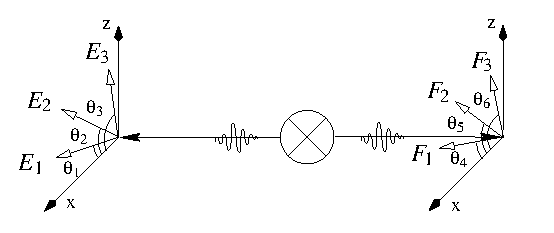
\includegraphics[width=90mm]{2003-qpoly-eifj}
  \caption{Measurements of spin components corresponding to the projections  ${E}_i$ and ${F}_j$.}
  \label{f-2003-qpoly-1}
\end{figure}
In such a case, the single-particle
 spin observables along $\theta$ correspond to the projections
$E_{i}$ and $F_{j}$; i.e.,
\begin{equation}
  \label{e-2003-qpoly-1}
E_i,F_j=E(\theta_i),F(\theta_j)=\frac{1}{2}({\Bbb I} +{\bf n}(\theta)\cdot{\bf \sigma})=
\frac{1}{2}\left(
  \begin{array}{cc}
    1 + \cos\theta& \sin\theta\\
    \sin\theta&1 - \cos\theta
    \end{array}
\right),
\end{equation}
where ${\bf \sigma}$ is a vector composed from Pauli spin matrices.

Any state operator $W$ must be self-adjoint $W^\dagger =W$,
of trace class ${\rm tr} (W)=1$, and  positive semidefinite
$\langle u | W | u \rangle \ge 0$ (in another
notation, $u^TWu\ge 0$) for all vectors $u\in H\otimes H$.
For the state to be pure, it must be a projector $W^2=W$,
or equivalently, ${\rm tr}(W^2)=1$.
In order to be able to parameterize $W$,
we recall (e.g., \cite[Sect. 72]{halmos-vs})
that a necessary and sufficient condition for
positiveness is its representation as the square of
some self-adjoint $B$; i.e., $W=B^2$.
In $n$ dimensions, $B$ can be parameterized by $n^2$
real independent parameters. Finally, $W$ can be normalized
by $W/ {\rm tr}(W)$.
Thus, for a two particle problem associated with $n=4$,
\begin{equation}
    \label{e-2003-qpoly-2}
    W={1 \over b_1+b_2+b_3+b_4}\left(\begin{array}{cccc}
        b_1 & b_5 + {\rm i}b_6 & b_{11} + {\rm i}b_{12} & b_{15} + {\rm i}b_{16}\\
        b_5 - {\rm i}b_6 & b_2 & b_7 + {\rm i}b_8 & b_{13} + {\rm i}b_{14}\\
        b_{11} - {\rm i}b_{12} & b_7 - {\rm i}b_8 & b_3 & b_9 + {\rm i}b_{10}\\
        b_{15} - {\rm i}b_{16} & b_{13} - {\rm i}b_{14} & b_9 - {\rm i}b_{10} &b_4
      \end{array}\right)^2
\end{equation}
for $b_1,b_2,\ldots ,b_{16}\in {\Bbb R}$.

The probability for finding the left particle in the spin-up state
along the angle $\theta$ is given  by
$q_i = {\rm tr}\{{W} [{E}(\theta_i) \otimes {\Bbb I}]\}$.
$q_j = {\rm tr}\{{W} [{\Bbb I} \otimes {F}(\theta_j)]\}$ is
the probability for finding the particle on the right hand side having
spin-up.
$q_{ij} = {\rm tr}\{{W} [{E}(\theta_i) \otimes {F}(\theta_j)]\}$ denotes the joint probability
for finding the left as well as the right particle in the spin-up state.
The associated expectation values are given by
$E(\alpha,\beta)={\rm tr}\{{W} [{\bf \sigma}_\alpha  \otimes
{\bf \sigma}_\beta ]\}$,
where $\sigma_\alpha= {\bf n}(\alpha )\cdot {\bf \sigma}$,
and ${\bf n}(\alpha ),{\bf n}(\beta )$
are unit vectors pointing in the directions
of spin measurement $\alpha$ and $\beta$, respectively.

We can utilize now the parameterizations of measurement operators
$E_i,\,F_j$ from Eq. (\ref{e-2003-qpoly-1})
and of states $W$ from Eq. (\ref{e-2003-qpoly-2})
to find violations of Boole-Bell-type
inequalities.
The general procedure is to choose a particular set of
projection operators and generate randomly arbitrary states $W$.
Having created a certain number of states, another set of
projection operators can be choosen as measurement operators.
A proper parameterization of the two sets representing samples of
measurement operators and states yields the basis
for expressing the maximal violations which reflect the quantum hull.


In a first step, we shall concentrate on the expectation values
rather than on probabilities.
Consider the CHSH-operator
$
  {\rm CHSH}(\alpha ,\beta ,\gamma ,\delta )=
\sigma_\alpha \sigma_\gamma + \sigma_\beta \sigma_\gamma +
  \sigma_\beta \sigma_\delta - \sigma_\alpha \sigma_\delta
$.
The quantum expectation values in
$ \|{\rm tr}[W\;{\rm CHSH}(\alpha ,\beta ,\gamma ,\delta )] \| = \|E(\alpha,\gamma) +
  E(\beta,\gamma) + E(\beta,\delta) - E(\alpha,\delta)\| \leq 2\sqrt{2}$
obey the Tsirelson bound
\footnote{Squaring ${\rm CHSH}$ yields  \cite[p. 174]{peres}
$
  {\rm CHSH}^2=4+[\sigma_\alpha,\sigma_\beta][\sigma_\gamma,\sigma_\delta]
$.
Since  for any two bounded
operators $A$ and $B$
$
  \|[A,B]\| \leq \|A B\| + \|B A\| \leq 2\|A\|\|B\|
$,
we obtain $\| {\rm CHSH}^2 \| \leq 8$ and hence
$  \|{\rm CHSH}\| \leq 2\sqrt{2}$.
}
for the configuration
$\alpha=0$,
$\beta=2\theta$,
$\gamma=\theta$,
$\delta=3\theta$ along $0 \le \theta \le \pi$.
(The classical CHSH-bound from above is $2$).
Its quantum hull is depicted in Figure  \ref{f-2003-qpoly-2}.
\begin{figure}[!ht]
  \centering
  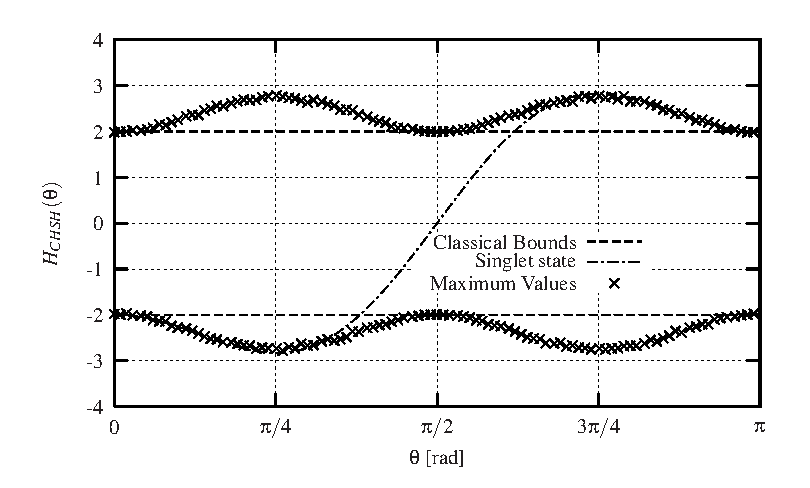
\includegraphics{2003-qpoly-plotchsh}
  \caption{The quantum hull of the CHSH operator.}
  \label{f-2003-qpoly-2}
\end{figure}


Next we shall study the quantum hull corresponding to the CH inequality
$ -1\leq p_{13} + p_{14} + p_{24} - p_{23} - p_{1} - p_{4} \leq 0$
which confines the classical probability sum inbetween $-1$ and $0$.
A one-parameter plot
can be obtained by restricting the projections
${E}_1(0)$, ${E}_2(\theta)={F}_1(\theta)$, ${F}_2(2\theta)$ to one parameter
$\theta$ variations.
In Figure  \ref{f-2003-qpoly-3} the quantum hull of CH
which is obtained by substituting $p$ through $q$ is plotted
along $0 \le \theta \le \pi$.
\begin{figure}
  \centering
  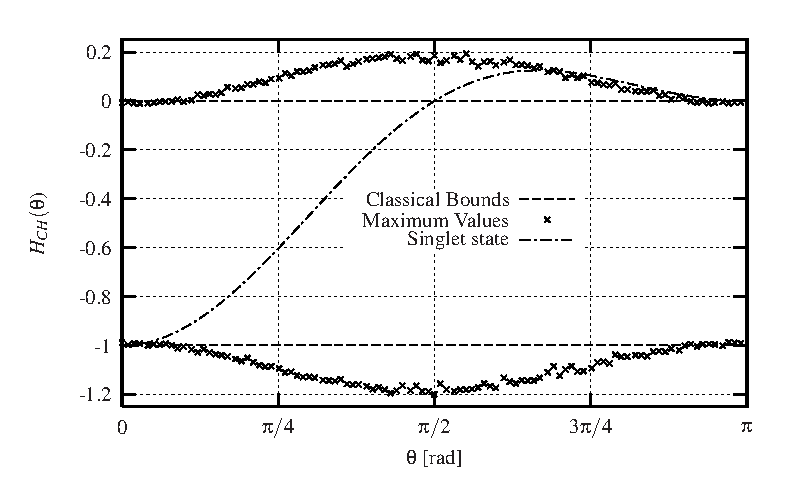
\includegraphics[clip]{2003-qpoly-plotch}
  \caption{Quantum hull associated with the CH-inequality}
  \label{f-2003-qpoly-3}
\end{figure}

As a third example, consider a quantum hull associated with the
configuration involving two spin 1/2 particles and
three measurement directions. One of the 684 Boole-Bell inequalities enumerated in
\cite{2000-poly} is
$  - p_{14} + p_{15} + p_{16} +
  p_{24} + p_{26} + p_{34} + p_{35} - p_{36} \leq +p_{1}+ p_{2} + p_{4} + p_{5}$.
The associated quantum operator is given by
\begin{equation}
\begin{array}{l}
  O=- {E}_1 \otimes {\Bbb I} - {E}_2 \otimes {\Bbb I} - {\Bbb I} \otimes {F}_1 - {\Bbb I} \otimes
  {F}_2 -
  {E}_1 \otimes {F}_1 + {E}_1 \otimes {F}_2 + {E}_1 \otimes {F}_3 +\\
\qquad \qquad {E}_2
  \otimes {F}_1 + {E}_2 \otimes {F}_3 +
  {E}_3 \otimes {F}_1 + {E}_3 \otimes {F}_2 - {E}_3 \otimes {F}_3.
\end{array}
  \label{e-2003-poly-xyz}
\end{equation}
By taking ${\rm tr}(WO)$ with
${E}_1={F}_1=E(0)$,
${E}_2={F}_2=E(\theta)$,
${E}_3={F}_3=E(2\theta)$, one obtains a quantum hull depicted in Figure  \ref{f-2003-plotpit}.
\begin{figure}
  \centering
  \includegraphics{2003-qpoly-plotpit}
  \caption{Quantum hull associated with the operator
${\rm tr}(WO)$ in Eq. (\ref{e-2003-poly-xyz}) as a function of the parameter
$\theta$ as ${E}_1={F}_1=E(0)$,
${E}_2={F}_2=E(\theta)$,
${E}_3={F}_3=E(2\theta)$.}
  \label{f-2003-plotpit}
\end{figure}

These three examples (Figure \ref{f-2003-qpoly-2}-\ref{f-2003-plotpit}) exhibit clearly that the quantum hull depends on
the measurement directions, i.~e. a particular set of
projection operators determines the maximal possible violation of a
Boole-Bell-type inequality although the choice of a state is only
restricted by fundamental quantum mechanical requirements.

So far we have seen certain quantum hulls associated with
the faces of classical correlation polytopes and bounds on expectation values,
but we have not depicted
``the real quantum thing'' yet; i.e., the convex body $Q$ itself.
In what follows, we shall get a glimpse of the quantum correlation polytope
for the two particle two measurement directions per particle configuration.
Classically, the CH polytope is bound by the $2^4$ vertices
$
(0,0,0,0,0,0,0,0)
$,
$
(0,1,0,0,0,0,0,0),
\ldots
(1,1,1,1,1,1,1,1)
$.
Consider a two-dimensional
cut through the polytope $c(2)$ by
$q_{1}=q_{2}=q_{3}=a$ and $q_{24}=c$, $a,c\ \mbox{const.}$.
More precisely, only those states and projection operators are chosen
with $q_{1}=q_{2}=q_{3}=a\pm\varepsilon$ and
$q_{24}=c\pm\varepsilon$ for some $a,c$. The probabilities $q_{13}$
and $q_{23}$ are also fixed to $q_{13}=q_{23}=b\pm\varepsilon$.
We now set $a=1/2$, $b=c=3/8$, and the tolerance $\varepsilon=\pm
0.015$. Figure \ref{f-2003-bell2hull}
depicts a projection of the quantum body $Q$ on
the plane spanned by $q_{4}$ and $q_{14}$.
\begin{figure}[htbp]
  \centering
  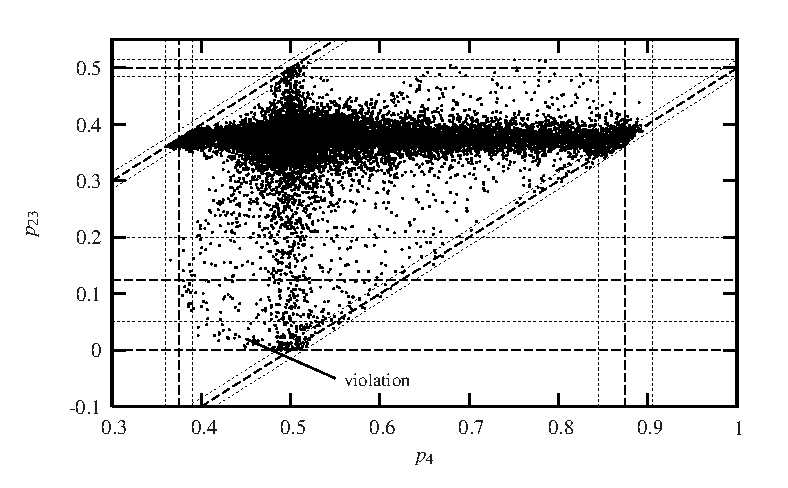
\includegraphics{2003-qpoly-bell2}
  \caption{Cut through the quantum body $Q$ for $a=1/2$, $b=c=3/8$, $\varepsilon=\pm 0.015$.}
  \label{f-2003-bell2hull}
\end{figure}


We conclude with the remark that
although the exact analytical
geometries of quantum bounds
remains unknown, our studies
reveal a fairly good estimate of its shapes.
We emphasize that these findings can be readily applied to experimental
tests of quantum theory, for no empirical
distribution should exceed these bounds imposed
by quantum probability theory.


%\bibliography{svozil}
%\bibliographystyle{apsrev}
%\bibliographystyle{unsrt}
%\bibliographystyle{plain}

\begin{thebibliography}{22}
\expandafter\ifx\csname natexlab\endcsname\relax\def\natexlab#1{#1}\fi
\expandafter\ifx\csname bibnamefont\endcsname\relax
  \def\bibnamefont#1{#1}\fi
\expandafter\ifx\csname bibfnamefont\endcsname\relax
  \def\bibfnamefont#1{#1}\fi
\expandafter\ifx\csname citenamefont\endcsname\relax
  \def\citenamefont#1{#1}\fi
\expandafter\ifx\csname url\endcsname\relax
  \def\url#1{\texttt{#1}}\fi
\expandafter\ifx\csname urlprefix\endcsname\relax\def\urlprefix{URL }\fi
\providecommand{\bibinfo}[2]{#2}
\providecommand{\eprint}[2][]{\url{#2}}

\bibitem[{\citenamefont{Boole}(1958)}]{Boole}
\bibinfo{author}{\bibfnamefont{G.}~\bibnamefont{Boole}},
  \emph{\bibinfo{title}{An investigation of the laws of thought}}
  (\bibinfo{publisher}{Dover edition}, \bibinfo{address}{New York},
  \bibinfo{year}{1958}).

\bibitem[{\citenamefont{Boole}(1862)}]{Boole-62}
\bibinfo{author}{\bibfnamefont{G.}~\bibnamefont{Boole}},
  \bibinfo{journal}{Philosophical Transactions of the Royal Society of London}
  \textbf{\bibinfo{volume}{152}}, \bibinfo{pages}{225} (\bibinfo{year}{1862}).

\bibitem[{\citenamefont{Bell}(1987)}]{bell-87}
\bibinfo{author}{\bibfnamefont{J.~S.} \bibnamefont{Bell}},
  \emph{\bibinfo{title}{Speakable and Unspeakable in Quantum Mechanics}}
  (\bibinfo{publisher}{Cambridge University Press},
  \bibinfo{address}{Cambridge}, \bibinfo{year}{1987}).

\bibitem[{\citenamefont{Clauser and Shimony}(1978)}]{clauser}
\bibinfo{author}{\bibfnamefont{J.~F.} \bibnamefont{Clauser}} \bibnamefont{and}
  \bibinfo{author}{\bibfnamefont{A.}~\bibnamefont{Shimony}},
  \bibinfo{journal}{Rep. Prog. Phys.} \textbf{\bibinfo{volume}{41}},
  \bibinfo{pages}{1881} (\bibinfo{year}{1978}).

\bibitem[{\citenamefont{Pitowsky}(1986)}]{pitowsky-86}
\bibinfo{author}{\bibfnamefont{I.}~\bibnamefont{Pitowsky}},
  \bibinfo{journal}{J. Math. Phys.} \textbf{\bibinfo{volume}{27}},
  \bibinfo{pages}{1556} (\bibinfo{year}{1986}).

\bibitem[{\citenamefont{Pitowsky}(1989{\natexlab{a}})}]{pitowsky}
\bibinfo{author}{\bibfnamefont{I.}~\bibnamefont{Pitowsky}},
  \emph{\bibinfo{title}{Quantum Probability---Quantum Logic}}
  (\bibinfo{publisher}{Springer}, \bibinfo{address}{Berlin},
  \bibinfo{year}{1989}{\natexlab{a}}).

\bibitem[{\citenamefont{Pitowsky}(1989{\natexlab{b}})}]{pitowsky-89a}
\bibinfo{author}{\bibfnamefont{I.}~\bibnamefont{Pitowsky}}, in
  \emph{\bibinfo{booktitle}{{B}ell's Theorem, Quantum Theory and the
  Conceptions of the Universe}}, edited by
  \bibinfo{editor}{\bibfnamefont{M.}~\bibnamefont{Kafatos}}
  (\bibinfo{publisher}{Kluwer}, \bibinfo{address}{Dordrecht},
  \bibinfo{year}{1989}{\natexlab{b}}), pp. \bibinfo{pages}{37--49}.

\bibitem[{\citenamefont{Pitowsky}(1991)}]{Pit-91}
\bibinfo{author}{\bibfnamefont{I.}~\bibnamefont{Pitowsky}},
  \bibinfo{journal}{Mathematical Programming} \textbf{\bibinfo{volume}{50}},
  \bibinfo{pages}{395} (\bibinfo{year}{1991}).

\bibitem[{\citenamefont{Pitowsky}(1994)}]{Pit-94}
\bibinfo{author}{\bibfnamefont{I.}~\bibnamefont{Pitowsky}},
  \bibinfo{journal}{Brit. J. Phil. Sci.} \textbf{\bibinfo{volume}{45}},
  \bibinfo{pages}{95} (\bibinfo{year}{1994}).

\bibitem[{\citenamefont{Froissart}(1991)}]{froissart-81}
\bibinfo{author}{\bibfnamefont{M.}~\bibnamefont{Froissart}},
  \bibinfo{journal}{Il Nuovo Cimento} \textbf{\bibinfo{volume}{64 B}},
  \bibinfo{pages}{241} (\bibinfo{year}{1991}).

\bibitem[{\citenamefont{Cirel'son}(1980)}]{cirelson:80}
\bibinfo{author}{\bibfnamefont{B.~S.} \bibnamefont{Cirel'son}},
  \bibinfo{journal}{Letters in Mathematical Physics}
  \textbf{\bibinfo{volume}{4}}, \bibinfo{pages}{93} (\bibinfo{year}{1980}).

\bibitem[{\citenamefont{{Cirel'son (=Tsirelson)}}(1993)}]{cirelson}
\bibinfo{author}{\bibfnamefont{B.~S.} \bibnamefont{{Cirel'son (=Tsirelson)}}},
  \bibinfo{journal}{Hadronic Journal Supplement} \textbf{\bibinfo{volume}{8}},
  \bibinfo{pages}{329} (\bibinfo{year}{1993}).

\bibitem[{\citenamefont{Ziegler}(1994)}]{ziegler}
\bibinfo{author}{\bibfnamefont{G.~M.} \bibnamefont{Ziegler}},
  \emph{\bibinfo{title}{Lectures on Polytopes}} (\bibinfo{publisher}{Springer},
  \bibinfo{address}{New York}, \bibinfo{year}{1994}).

\bibitem[{\citenamefont{Pitowsky and Svozil}(2001)}]{2000-poly}
\bibinfo{author}{\bibfnamefont{I.}~\bibnamefont{Pitowsky}} \bibnamefont{and}
  \bibinfo{author}{\bibfnamefont{K.}~\bibnamefont{Svozil}},
  \bibinfo{journal}{Physical Review} \textbf{\bibinfo{volume}{A64}},
  \bibinfo{pages}{014102} (\bibinfo{year}{2001}), \eprint{quant-ph/0011060}.

\bibitem[{\citenamefont{Filipp and Svozil}(2001)}]{2001-cddif}
\bibinfo{author}{\bibfnamefont{S.}~\bibnamefont{Filipp}} \bibnamefont{and}
  \bibinfo{author}{\bibfnamefont{K.}~\bibnamefont{Svozil}}
  (\bibinfo{year}{2001}), \bibinfo{note}{e-print {\tt arXiv:quant-ph/0105083}
  available {http://arxiv.org/abs/quant-ph/0105083}}.

\bibitem[{\citenamefont{Popescu and Rohrlich}(1994)}]{pop-rohr}
\bibinfo{author}{\bibfnamefont{S.}~\bibnamefont{Popescu}} \bibnamefont{and}
  \bibinfo{author}{\bibfnamefont{D.}~\bibnamefont{Rohrlich}},
  \bibinfo{journal}{Foundations of Physics} \textbf{\bibinfo{volume}{24}},
  \bibinfo{pages}{379} (\bibinfo{year}{1994}).

\bibitem[{\citenamefont{Krenn and Svozil}(1998)}]{svozil-krenn}
\bibinfo{author}{\bibfnamefont{G.}~\bibnamefont{Krenn}} \bibnamefont{and}
  \bibinfo{author}{\bibfnamefont{K.}~\bibnamefont{Svozil}},
  \bibinfo{journal}{Foundations of Physics} \textbf{\bibinfo{volume}{28}},
  \bibinfo{pages}{971} (\bibinfo{year}{1998}).

\bibitem[{\citenamefont{Khalfin and Tsirelson}(1992)}]{khalfin-97}
\bibinfo{author}{\bibfnamefont{L.~A.} \bibnamefont{Khalfin}} \bibnamefont{and}
  \bibinfo{author}{\bibfnamefont{B.~S.} \bibnamefont{Tsirelson}},
  \bibinfo{journal}{Foundations of Physics} \textbf{\bibinfo{volume}{22}},
  \bibinfo{pages}{879} (\bibinfo{year}{1992}).

\bibitem[{\citenamefont{Pitowsky}(2002)}]{pit:range-2001}
\bibinfo{author}{\bibfnamefont{I.}~\bibnamefont{Pitowsky}}, in
  \emph{\bibinfo{booktitle}{Quantum Theory: Reconsideration of Foundations,
  Proceeding of the 2001 Vaxjo Conference}} (\bibinfo{publisher}{World
  Scientific}, \bibinfo{address}{Singapore}, \bibinfo{year}{2002}),
  \eprint{quant-ph/0112068}.

\bibitem[{\citenamefont{Fishburn and Reeds}(1994)}]{fishburn-reeds-1994}
\bibinfo{author}{\bibfnamefont{P.~C.} \bibnamefont{Fishburn}} \bibnamefont{and}
  \bibinfo{author}{\bibfnamefont{J.~A.} \bibnamefont{Reeds}},
  \bibinfo{journal}{SIAM J. Disc. Math.} \textbf{\bibinfo{volume}{7}},
  \bibinfo{pages}{48} (\bibinfo{year}{1994}).

\bibitem[{\citenamefont{Halmos}(1974)}]{halmos-vs}
\bibinfo{author}{\bibfnamefont{P.~R.} \bibnamefont{Halmos}},
  \emph{\bibinfo{title}{Finite-Dimensional Vector spaces}}
  (\bibinfo{publisher}{Springer}, \bibinfo{address}{New York, Heidelberg,
  Berlin}, \bibinfo{year}{1974}).

\bibitem[{\citenamefont{Peres}(1993)}]{peres}
\bibinfo{author}{\bibfnamefont{A.}~\bibnamefont{Peres}},
  \emph{\bibinfo{title}{Quantum Theory: Concepts and Methods}}
  (\bibinfo{publisher}{Kluwer Academic Publishers},
  \bibinfo{address}{Dordrecht}, \bibinfo{year}{1993}).

\end{thebibliography}

\end{document}
